\subsection{\texorpdfstring{阿廷环的格罗滕迪克群 \(K_{0}(A)\)}{阿廷环的格罗滕迪克群 K\_\{0\}(A)}}

设 A 是一个左阿廷环。用 r 表示它的根；它是 A 的一个幂零双边理想，且环 A/r 是半单的（VIII, 第 173 页，命题 1）。由 VIII, 第 176 页的推论，映射 P \(\mapsto\) cl(P/rP) 是从幺半群 \(\mathcal{P}(A)\) 到幺半群 \(\mathcal{P}(A/r)\) 的一个同构。由此我们导出一个群同构 \(\gamma\)，它从 \(K_{0}(A)\) 到 \(K_{0}(A/r)\)，由关系式 \(\gamma([\mathrm{P}]_{\mathcal{P}(A)}) = [\mathrm{P}/\mathfrak{r}\mathrm{P}]_{\mathcal{P}(A/r)}\)（对每个有限生成投射 A-模 P）刻画。

由于环 A/r 是半单的，上面的注蕴含等式 \(\mathrm{R}(\mathrm{A}/\mathfrak{r}) = \mathrm{K}_{0}(\mathrm{A}/\mathfrak{r})\)。环 A/r 上的有限长度模就是环 A 上的有限长度半单模（VIII, 第 174 页，命题 2）；因此，我们可以把 \(\mathcal{L}\mathcal{F}(\mathrm{A}/\mathfrak{r})\) 与 \(\mathcal{S}\mathcal{S}(\mathrm{A})\) 等同，把 \(\mathrm{R}(\mathrm{A}/\mathfrak{r})\) 与 \(\mathrm{K}(\mathcal{S}\mathcal{S}(\mathrm{A}))\) 等同。我们用 \(\delta\) 表示同态 \(\gamma_{\mathcal{L}\mathcal{F}(\mathrm{A}),\mathcal{S}\mathcal{S}(\mathrm{A})}\)，它从 \(\mathrm{R}(\mathrm{A}/\mathfrak{r}) = \mathrm{K}(\mathcal{S}\mathcal{S}(\mathrm{A}))\) 到 \(\mathrm{R}(\mathrm{A}) = \mathrm{K}(\mathcal{L}\mathcal{F}(\mathrm{A}))\)（VIII, 第 191 页，注 1）；它是一个同构。最后，我们有 \(\mathcal{P}(\mathrm{A}) \subset \mathcal{L}\mathcal{F}(\mathrm{A})\)，并且令 \(\varepsilon =\) \(\gamma_{\mathcal{L}\mathcal{F}(\mathrm{A}),\mathcal{P}(\mathrm{A})}\)。我们已定义了一个图表

\pandocbounded{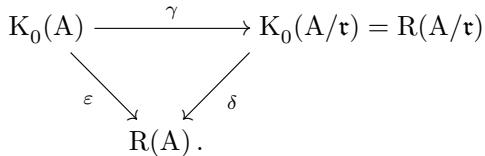
\includegraphics[keepaspectratio]{images/part002_05770a86.jpg}}

我们用 \(\mathcal{S}\) 表示单 A-模的类所成之（有限）集；对每个 \(\lambda \in \mathcal{S}\)，选取一个模 \(S_{\lambda}\)（其类为 \(\lambda\)）和一个投射覆盖 \((P_{\lambda}, u_{\lambda})\)（它覆盖 \(S_{\lambda}\)）（VIII, 第 175 页，命题 4）。由 VIII, 第 176 页的命题 6 得出，\(K_0(A)\) 是一个自由 \(\mathbf{Z}\)-模，以族 \(([P_{\lambda}]_{\mathcal{P}(A)})_{\lambda \in \mathcal{S}}\) 为基。此外，由于 \(S_{\lambda}\) 同构于 \(P_{\lambda} / \mathfrak{r}P_{\lambda}\)（VIII, 第 176 页），\(\gamma\) 把基 \(([P_{\lambda}]_{\mathcal{P}(A)})_{\lambda \in \mathcal{S}}\)（\(K_0(A)\) 的基）变为基 \(([S_{\lambda}])_{\lambda \in \mathcal{S}}\)（\(R(A / \mathfrak{r})\) 的基）。同构 \(\delta\) 把基 \(([S_{\lambda}])_{\lambda \in \mathcal{S}}\)（\(R(A / \mathfrak{r})\) 的基）变为基 \(([S_{\lambda}])_{\lambda \in \mathcal{S}}\)（\(R(A)\) 的基）。

A 的嘉当矩阵是矩阵 \((a_{\lambda\mu})\)，即 Z-模同态 \(\varepsilon: K_{0}(A) \to R(A)\) 关于基 \(([P_{\lambda}]_{\mathcal{P}(A)})_{\lambda \in \mathcal{S}}\)（\(K_{0}(A)\) 的基）与基 \(([S_{\lambda}])_{\lambda \in \mathcal{S}}\)（\(R(A)\) 的基）的矩阵。按定义，我们有

\[
[ \mathrm{P} _ {\mu} ] = \sum_ {\lambda \in \mathcal {S}} a _ {\lambda \mu} [ \mathrm{S} _ {\lambda} ] \quad (\mu \in \mathcal {S})\tag{19}
\]

（在群 R(A) 中）。换句话说，\(a_{\lambda\mu}\) 是同构于 \(S_{\lambda}\) 的商在 A-模 \(P_{\mu}\) 的某条若尔当–赫尔德列中的个数。

令 \(\pi = \varepsilon \circ \gamma^{-1} \circ \delta^{-1}\)；它是群 R(A) 的一个自同态。若 M 是一个有限生成半单 A-模且 (P, \(u\)) 是 M 的一个投射覆盖，则我们有 \(\pi([M]) = [P]\)。由公式 (19)，\(\pi\) 关于 R(A) 的基 \(([S_{\lambda}])_{\lambda \in \mathcal{S}}\) 的矩阵正是 A 的嘉当矩阵。

